\chapter{Experiments and Results}
\section{Scaling}

Scaling Up a Baseline Model with Different Network Width (w), Depth (d), and Resolution (r) Coefficients. Bigger networks with larger width, depth, or resolution tend to achieve higher accuracy, but the accuracy gain quickly saturate after reaching 80%, demonstrating the limitation of single dimension scaling. Baseline network is described as described below.

\begin{figure}[htpb]
\centering
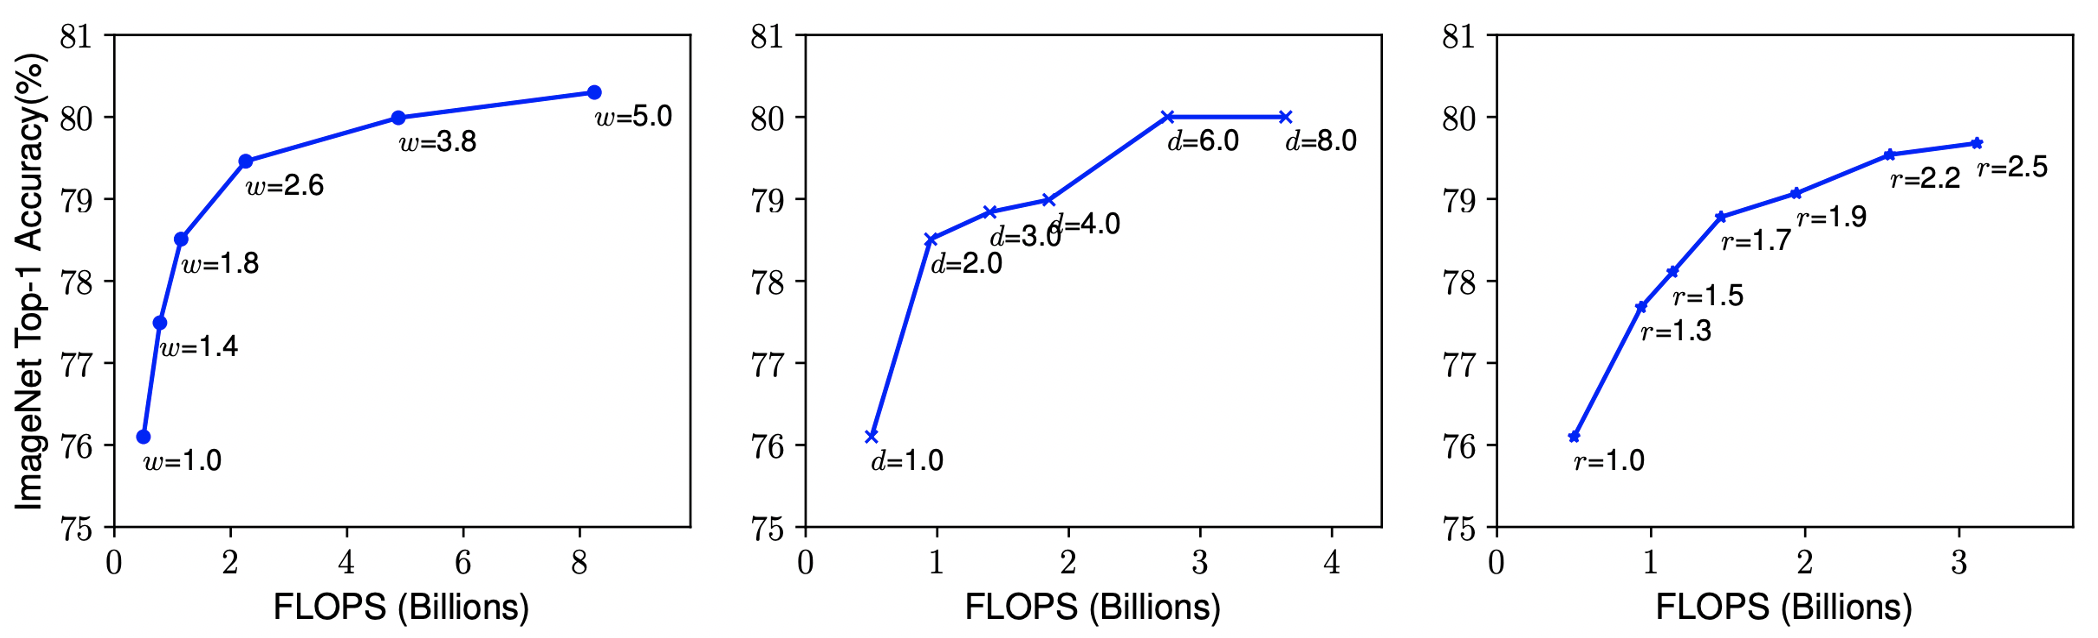
\includegraphics[width=\textwidth,height=\textheight,keepaspectratio]{../../static/Depth Scaling.png}
\caption{Depth Scaling.png}
\end{figure}Scaling Network Width for Different Baseline Networks. Each dot in a line denotes a model with different width coefficient (w). All baseline networks are from the previous table. The first baseline network (d=1.0, r=1.0) has 18 convolutional layers with resolution 224x224, while the last baseline (d=2.0, r=1.3) has 36 layers with resolution 299x299.

\begin{figure}[htpb]
\centering
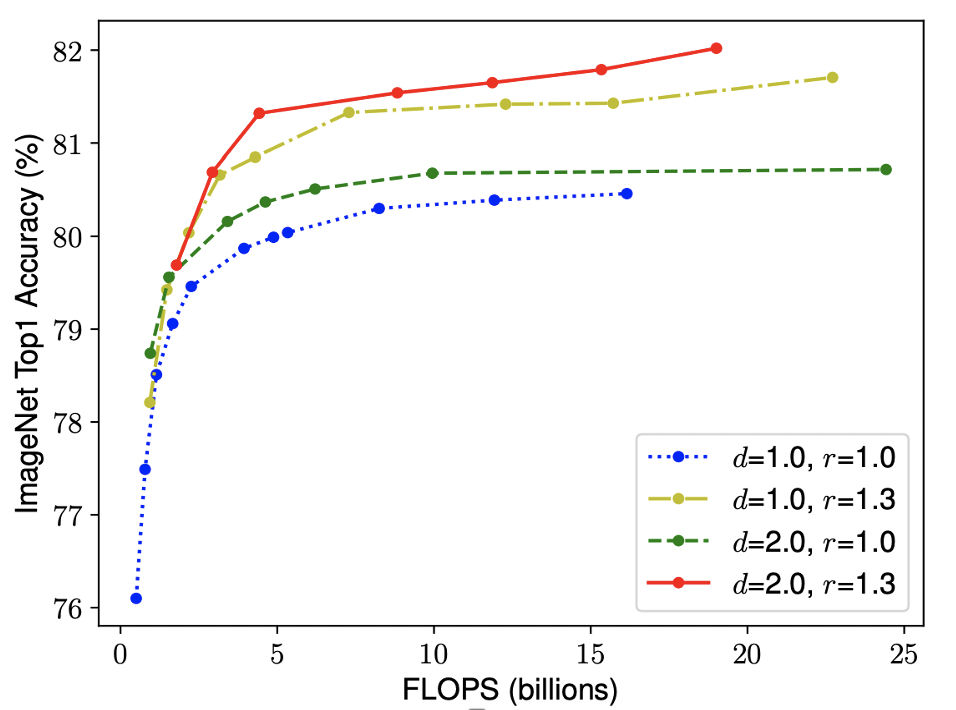
\includegraphics[width=\textwidth,height=\textheight,keepaspectratio]{../../static/Scaling Depth and Resolution.png}
\caption{Scaling Depth and Resolution.png}
\end{figure}
\section{Comparison of EffecientNet}

As seen in the figure, the scaled models use upto 8.4x less parameters and a total reduction of upto 16x FLOPS is observed. The models were compared head-to-head against state of the art networks in their respective tasks.

\begin{figure}[htpb]
\centering
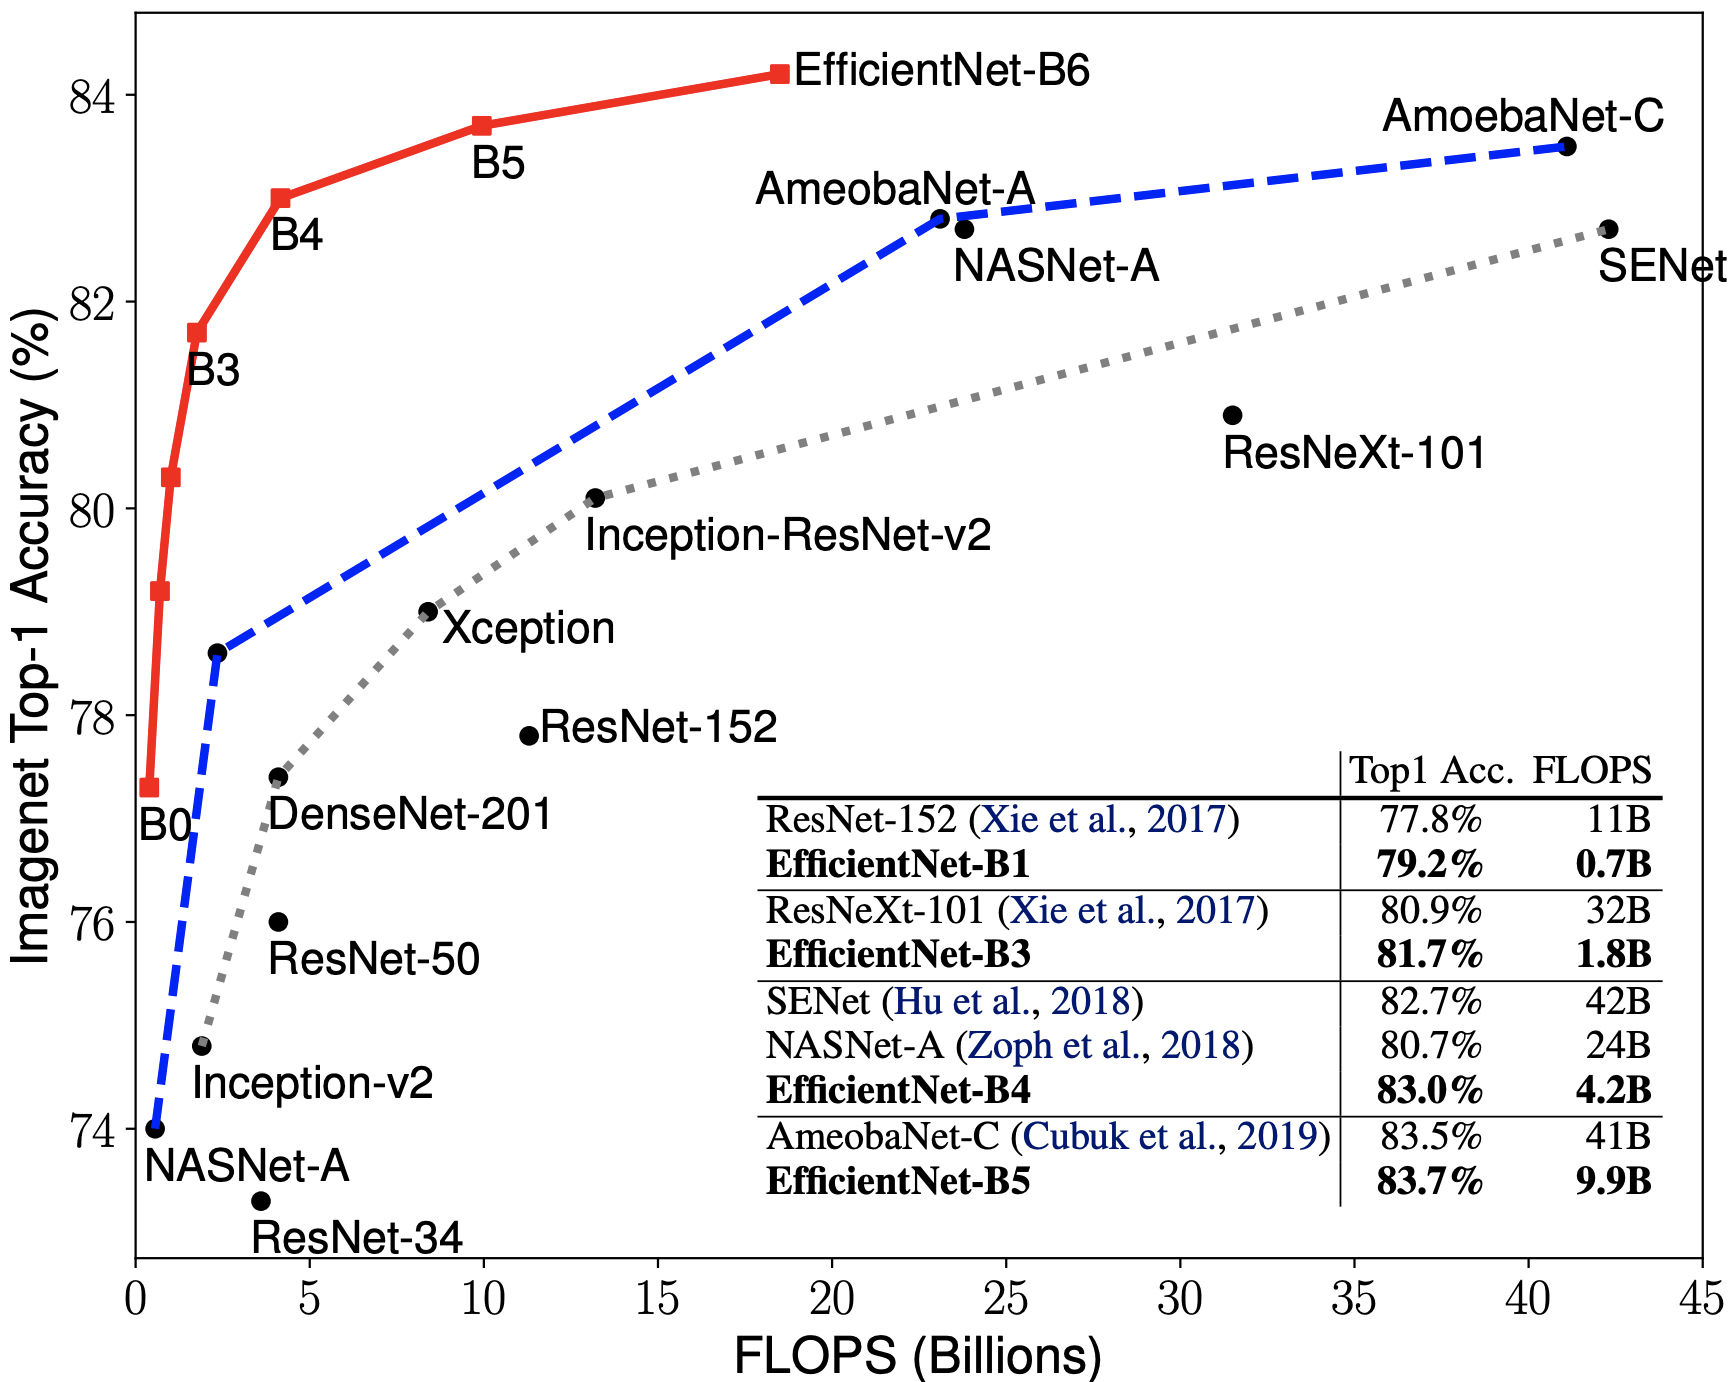
\includegraphics[width=\textwidth,height=\textheight,keepaspectratio]{../../static/Results.png}
\caption{Results.png}
\end{figure}It is also very evident that the compound scaling method also improves CNN dependability as we can see that the CNN is now focusing on the required objects for the task in a more accurate manner. This is done by freezing the training at an intermediate step and then observing one of the layers of the CNN. This demonstrates the ability of this algorithm to also apply to transfer learning tasks with good performance. Hence we can use these modified networks in mobile devices with less computing power but with the same efficiency of the full size model.
\begin{figure}[htpb]
\centering
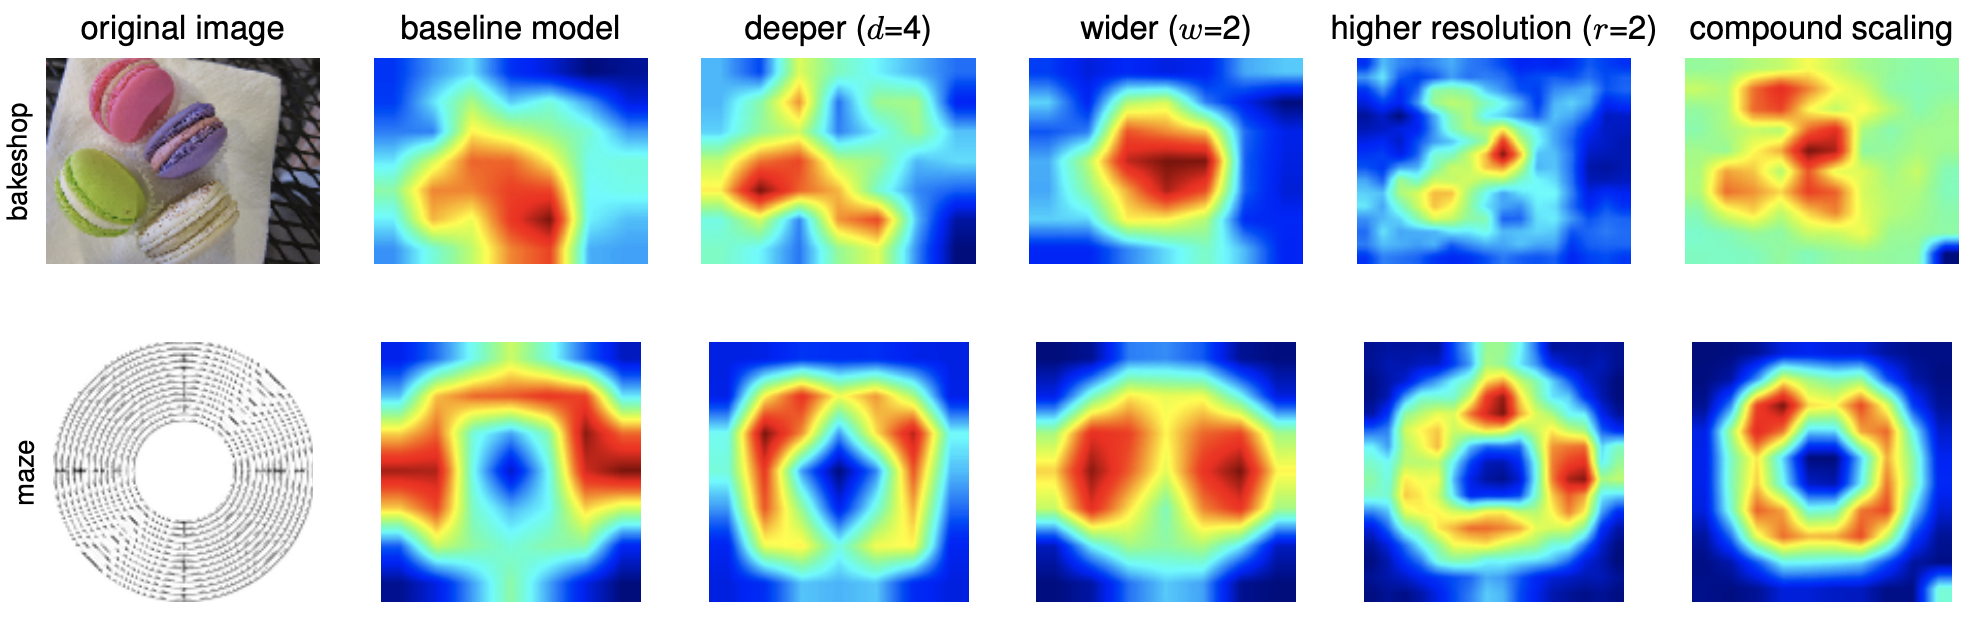
\includegraphics[width=\textwidth,height=\textheight,keepaspectratio]{../../static/What the network can see.png}
\caption{What the network can see.png}
\end{figure}
\section{Limitations}

It is possible to achieve even better performance by searching for alpha, beta and gamma directly around a large model, but the search cost becomes prohibitively more expensive on larger model. Hence we would require much higher computation power for doing such a task.
